\section{Experimental Evaluation}
\label{sec:exp}

\begin{figure*}[t!]
\centering
\begin{minipage}{3.3in}
  \centering
  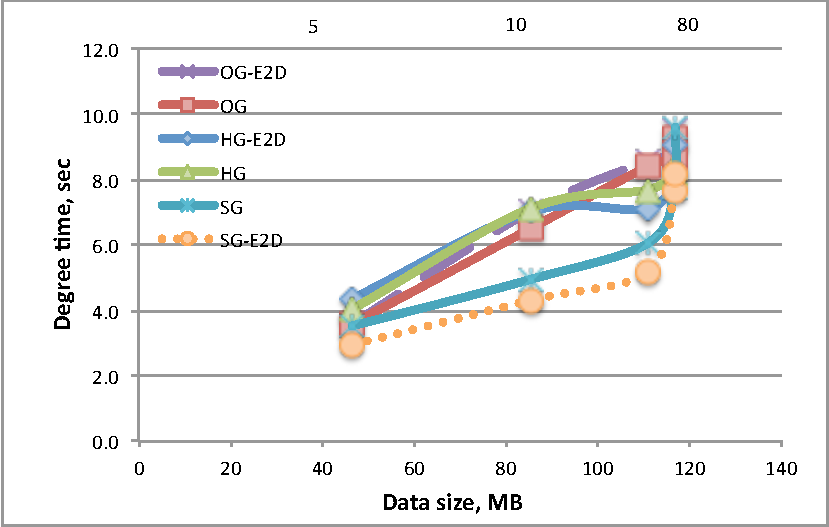
\includegraphics[width=2.8in]{figs/degrees_dblp.pdf}
  \vspace{-0.1in}
  \caption{Degrees time, DBLP.}
  \label{fig:deg_dblp}
  \vspace{-0.1in}
\end{minipage}
\begin{minipage}{3.3in}
  \centering
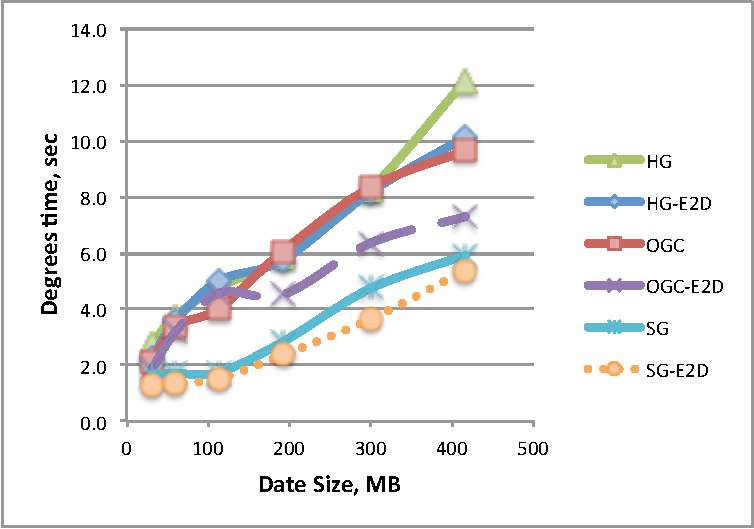
\includegraphics[width=2.8in]{figs/degrees_ngrams.pdf}
  \vspace{-0.1in}
\caption{Degrees time, nGrams.}
\label{fig:deg_ngrams}
  \vspace{-0.1in}
\end{minipage}
\end{figure*}

\begin{figure*}[t]
\centering
\begin{minipage}{3.3in}
  \centering
  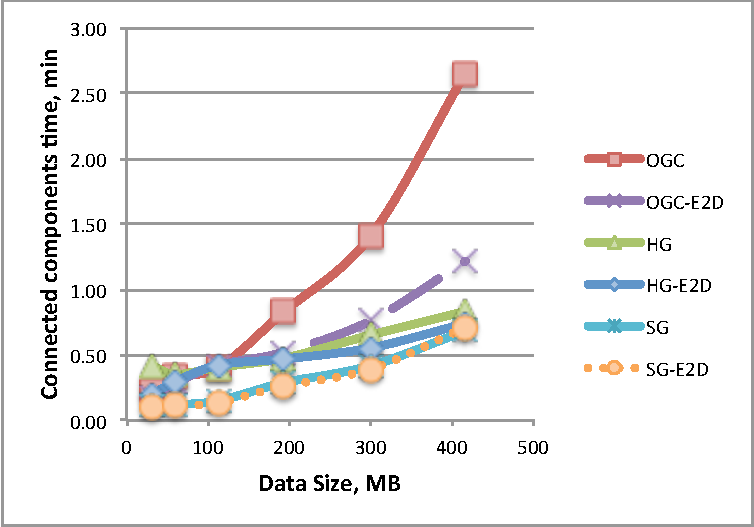
\includegraphics[width=2.8in]{figs/connectedcs_ngrams.pdf}
  \vspace{-0.1in}
  \caption{Connected Components, nGrams.}
  \label{fig:connectc_ngrams}
  \vspace{-0.5cm}
\end{minipage}
\begin{minipage}{3.3in}
  \centering
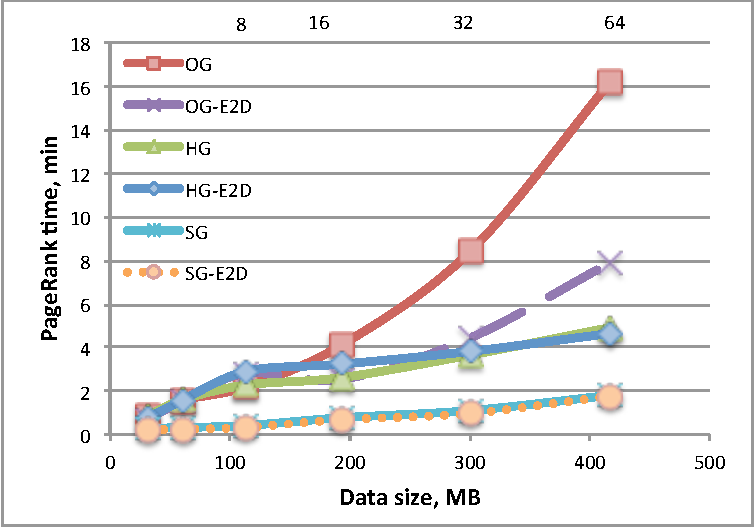
\includegraphics[width=2.8in]{figs/pagerank_ngrams.pdf}
  \vspace{-0.1in}
\caption{PageRank, nGrams.}
\label{fig:pagerank_ngrams}
  \vspace{-0.5cm}
\end{minipage}
\end{figure*}

{\bf Experimental environment.} All experiments in this section were
conducted on an 8-slave in-house Open Stack cloud, using Linux Ubuntu
14.04 and Spark v1.4.  Each node has 4 cores and 16 GB of RAM.  Spark
Standalone cluster manager and Hadoop 2.6 were used.

Because Spark is a lazy evaluation system, a \insql{materialize}
operation was appended to the end of each query, which consisted of
the count of nodes and edges.  In cases where the goal was to evaluate
a specific operation in isolation, we used warm start, which consisted
of materializing the graph upon load.  Each experiment was conducted 3
times, we report the average running time, which is representative
because we took great care to control variability.  Standard deviation
for each measure is at or below 5\% of the mean except in cases of
very small running times.

{\bf Data.}  We evaluate performance of our framework on two real
open-source datasets.
%\begin{enumerate}%[leftmargin=*]
%\item 
DBLP\footnote{\url{http://dblp.uni-trier.de/}} is a 250 MB dataset
that contains co-authorship information from 1936 through 2015, with
over 1.5 million author nodes and over 6 million undirected
co-authorship edges.
%
nGrams\footnote{\url{http://storage.googleapis.com/books/ngrams/books/datasetsv2.html}}
is a 40 GB dataset that contains word co-occurrences from 1520 through
2008, with over 1.5 million word nodes and over 65 million undirected
co-occurrence edges.

The nGrams dataset is of comparable size to the LiveJournal dataset
in~\cite{Xin2013} and is commensurate with our cluster size.  DBLP and
nGrams differ not only in size, but also in the evolutionary
properties: co-authorship network nodes and edges have limited
lifespan, while the nGrams network grows over time, with nodes and
edges persisting for long duration.  \eat{All figures in the body of
  this section are on the larger nGrams dataset.  Refer to the
  Appendix for the DBLP figures, which show similar trends as nGrams.}
We plan to experiment with a larger DELIS
\eat{\footnote{\url{law.di.unimi.it/webdata/uk-union-2006-06-2007-05}}}
dataset~\cite{BoVWFI} as we grow our cluster in the near future.

%\subsection{Degrees}

{\bf Degrees.} Computation of the number of edges for each vertex is
performed using a single round of messages between nodes, with batch
mode for HG and OG.  We used the following query to evaluate data
structure performance over varying number of snapshots:

\begin{small}
\begin{verbatim}
      TSelect V[vid, degrees()]; E[vid1, vid2]
      From    nGrams
      TWhere  Start >= :x And End < :y
\end{verbatim}
\end{small}

Results of this experiment are presented in Figures~\ref{fig:deg_dblp}
and~\ref{fig:deg_ngrams}, both with warm start.  Observe that SG
outperforms HG and OG for smaller data sizes.  This is contrary to our
expectation that batch mode of HG and OG would always be faster than
SG.  SG performance can be explained if we consider that each snapshot
is spread out over fewer partitions than in the aggregate data
structures.  Thus, more communication occurs intra-partition rather
than between partitions, which in turn dominates the overall running
time.  Furthermore, we expected HG performance to be between SG and
OG, the two data structures that it combines.  We do observe this in
most cases, but not consistently.  We believe that HG does not
consistently outperform OG due to its sensitivity to temporal skew.
This effect is particularly pronounced for fast-running operations
like Degree.

%\subsection{Connected Components}

{\bf Connected components.} Snapshot analytics like Connected
Components are implemented using the Pregel API in GraphX, with batch
mode for HG and OG.  The algorithm was executed until convergence,
with no limit to the number of iterations.  We used the following
query to evaluate data structure performance over varying number of
snapshots:

\begin{small}
\begin{verbatim}
      TSelect V[vid, components()]; E[vid1, vid2]
      From    nGrams
      TWhere  Start >= :x And End < :y
\end{verbatim}
\end{small}

\eat{ Performance of Pregel-based algorithms depends heavily on the
  partition strategy, with best results achieved where cross-partition
  communication is small.  For this reason, we evaluated only no
  partitioning and E2D.}

SG performs better than the other data structures in this experiment,
contrary to our expectation that batch mode of HG and OG would be
faster (Figure~\ref{fig:connectc_ngrams}).  This can be explained by
HG and OG using significantly more cross-partition communication due
to the following factors:

\begin{figure*}[t!]
\centering
\begin{minipage}{3.3in}
  \centering
  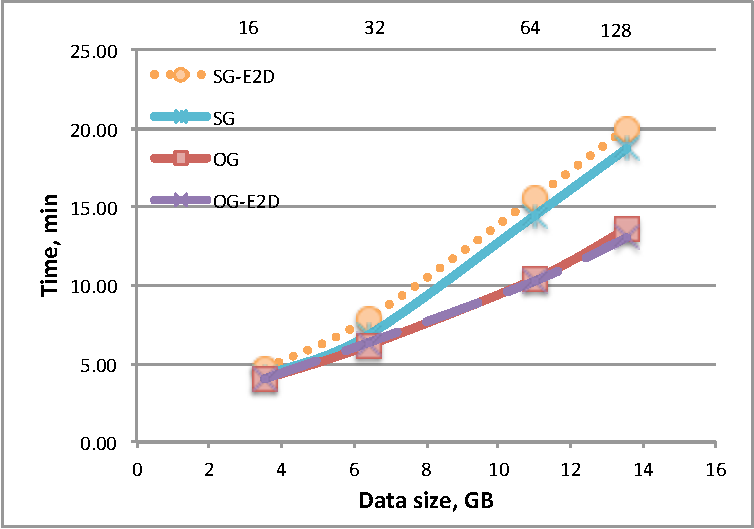
\includegraphics[width=2.8in]{figs/trend_degrees.pdf}
  \vspace{-0.1in}
  \caption{\insql{trend(degrees())}.}
  \label{fig:trend_deg}
  \vspace{-0.5cm}
\end{minipage}
\begin{minipage}{3.3in}
  \centering
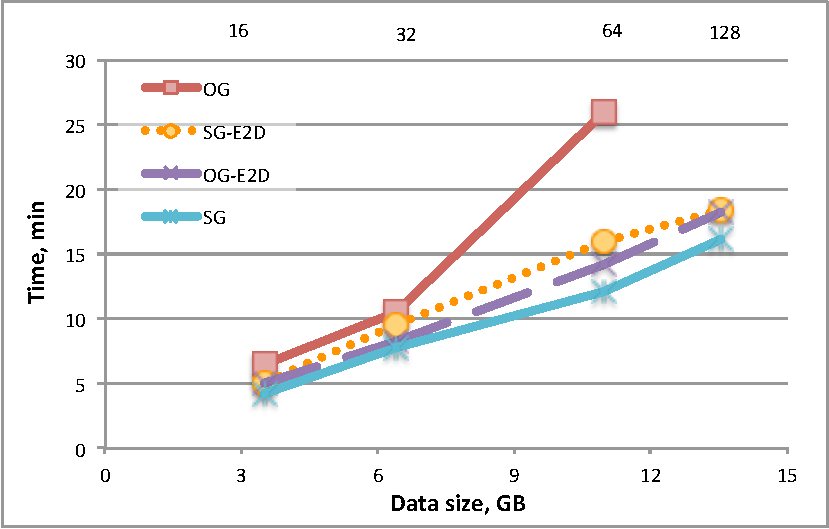
\includegraphics[width=2.8in]{figs/complexq.pdf}
  \vspace{-0.1in}
\caption{\insql{TGroup}, PageRank, trend.}
\label{fig:complexq}
  \vspace{-0.5cm}
\end{minipage}
\end{figure*}

\begin{enumerate}[leftmargin=*]
\item Each individual snapshot is less dense than the aggregate
  (although this depends on the rate of change), and dense graphs do
  worse with Pregel analytics.
\item Individual snapshots are smaller and take fewer partitions, so
  less communication happens across partitions.
\item Iterations get faster as vertex values converge, and vertices
  stop sending messages.  In OG/HG, a vertex converges only when it
  does so in all represented snapshots.
\end{enumerate}

However, note that as the number of total snapshots increases, HG
performance improves compared to SG, and in fact for the largest size
(128 snapshots) HG surpasses SG in performance.  We saw this trend in
both data sets.

%\subsection{PageRank}

{\bf PageRank.} Like Connected Components, PageRank is implemented
using Pregel.  The query in this experiment is the same, replacing
\insql{components} with \insql{pagerank}.  PageRank was executed for
10 iterations or until convergence, whichever came first.  Results of
this experiment (Figure~\ref{fig:pagerank_ngrams}) are similar to
those of Connected Components.  SG outperforms the other data
structures, but HG exhibits the same slope and its performance
improves relative to the other data structures as the number of
snapshots is increased.  E2D partitioning leads to performance
improvements for SG, but inconsistent for HG/OG.

%\subsection{Mixed queries}

{\bf Mixed queries.} All the experiments so far evaluated performance
of individual \ql snapshot analytics operations.  Our final experiment
considers performance of snapshot and trend analytics that are
executed as part of a query that also includes temporal selection
(\insql{TWhere}) and aggregation (\insql{TGroup}).  Note that we do
not currently have an implementation of temporal aggregation for HG,
and so HG is not used in this experiment.

\begin{small}
\begin{verbatim}
 TSelect V[vid, trend(deg)]; E
 From    (TSelect V[vid, degrees() as deg]; E[vid1, vid2]
          From    nGrams
          TWhere  Start >= :x And End < :y)
 TGroup  by 16 years
\end{verbatim}
\end{small}

This query computes the degree of each vertex in each snapshot,
aggregates snapshots in groups of 16, and uses \insql{trend} as the
aggregation function on degrees.  We have shown above that in most
cases SG provides the most efficient performance for snapshot
analytics.  We have also shown in~\cite{PortalarXiv2016} that
aggregate data structures (OG, HG, others) take longer to load but are
more efficient for \insql{TGroup}.  Figure~\ref{fig:trend_deg} (warm
start) shows that, when these operations are combined, OG outperforms
SG.  Temporal aggregation is a more expensive operation in this
scenario that the degrees analytic.

\eat{
\subsection{\insql{TSelect} with \insql{trend(pagerank())}}
}

We conclude this section with a cold-start execution of
the following SQL-\ql query:

\begin{small}
\begin{verbatim}
 Select vid, pr
 From (TSelect V[vid, trend(prank) as pr];  E
       From (TSelect All V[vid, pagerank() as prank]; 
                     All E
             From nGrams
             TWhere Start >= :x And End < :y
             TGroup by 16 years)
      TGroup by size).toVerticesFlat()
 Order by pr
 Limit 10
\end{verbatim}
\end{small}

\eat{ As we saw above, SG outperforms other representations for data
  load and for PageRank, while OGC is very efficient for temporal
  aggregation.  This query combines all of these operations, and adds
  a trend analytic, and a transformation of the vertices of the result
  into a flat vertex relation.  } 

Here, SG with no partitioning, and OG with E2D show comparable
performances, as seen in Figure~\ref{fig:complexq}.

\eat{
\begin{figure}[t]
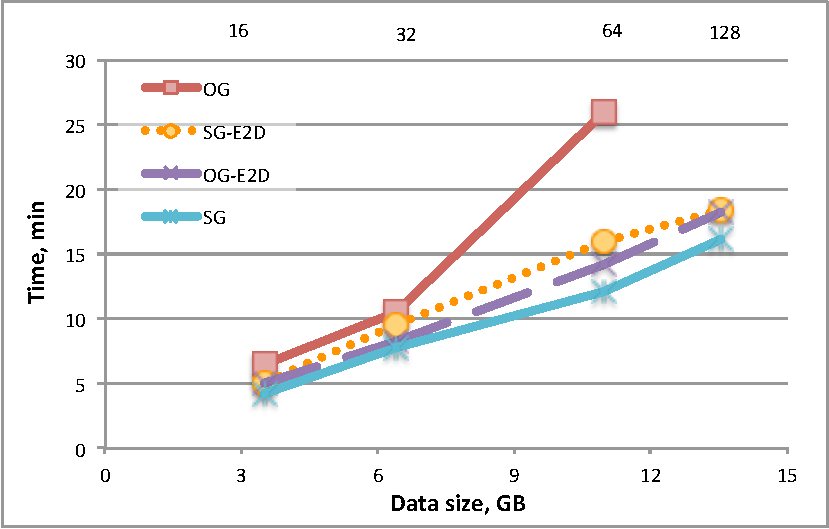
\includegraphics[width=3.2in]{figs/complexq.pdf}
\caption{Complex query: \insql{TGroup}, PageRank, trend.}
\label{fig:complexq}
\end{figure}
}

{\bf In summary,} running times of the best-performing data structure
for each experiment are reasonable, and show a linear trend with
increasing data size.  Interestingly, no one data structure is most
efficient across all operations.  \eat{SG is most efficient for data
  load, because our file format favors this data structure, and for
  PageRank.  OGC is most efficient for temporal group and join.  The
  two data structures perform comparably for the complex query.  E2D
  is the most efficient partitioning method in most cases, and
  E2D-Temporal is a close second.}  SG is most efficient for snapshot
analytics in most cases, but HG outperforms it for larger data sizes,
while OG provides a good balance for mixed queries.  These insights
motivate future work on query optimization in \ql.
